\documentclass[12pt,letterpaper]{article}
\usepackage[margin=1in]{geometry}
\usepackage{amsmath}
\usepackage{amsfonts}
\usepackage{amssymb}
\usepackage{graphicx}
\usepackage{tikz}
\usepackage{circuitikz}
\usepackage{pgfplots}
\usepackage{siunitx}
\usepackage{float}
\usepackage{subcaption}
\usepackage{fancyhdr}
\usepackage{hyperref}

\usetikzlibrary{shapes,arrows,positioning,calc,decorations.pathmorphing,patterns}
\usetikzlibrary{decorations.markings}
\pgfplotsset{compat=1.16}

% Define block diagram styles
\tikzstyle{block} = [draw, fill=blue!20, rectangle, minimum height=3em, minimum width=6em]
\tikzstyle{sum} = [draw, fill=blue!20, circle, node distance=1cm]
\tikzstyle{input} = [coordinate]
\tikzstyle{output} = [coordinate]
\tikzstyle{pinstyle} = [pin edge={to-,thin,black}]

% Page formatting
\pagestyle{fancy}
\fancyhf{}
\rhead{Control Systems Diagrams}
\lhead{Mechanical Systems}
\cfoot{\thepage}

\title{Free Body Diagrams and Control System Block Diagrams\\for Mechanical Systems}
\author{Control Systems Modeling}
\date{\today}

\begin{document}

\maketitle

\tableofcontents
\newpage

\section{Introduction}

This document presents comprehensive free body diagrams and control system block diagrams for various mechanical systems commonly encountered in control systems engineering. Each system is analyzed with its governing equations, free body diagram, and corresponding control system representation.

\section{Servo Motor System}

\subsection{System Description}

A servo motor system consists of a DC motor with moment of inertia $J$, damping coefficient $D$, and torque constant $K_t$. The motor current $I$ generates torque to rotate the shaft.

\subsection{Governing Equation}

\begin{equation}
J\ddot{\theta} + D\dot{\theta} = K_t I
\end{equation}

where:
\begin{itemize}
    \item $J$ = moment of inertia (kg·m²)
    \item $D$ = damping coefficient (N·m·s/rad)
    \item $K_t$ = torque constant (N·m/A)
    \item $I$ = motor current (A)
    \item $\theta$ = angular position (rad)
\end{itemize}

\subsection{Free Body Diagram}

\begin{figure}[H]
\centering
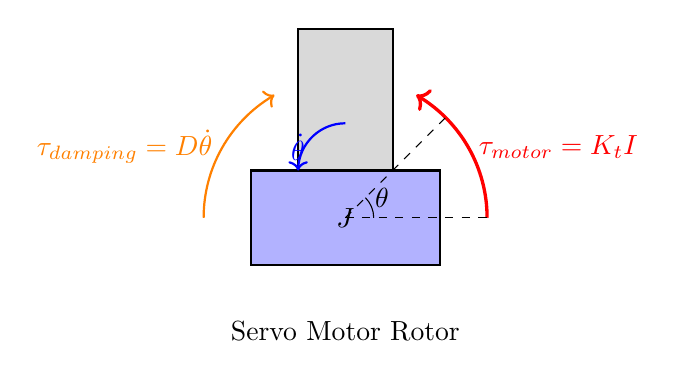
\begin{tikzpicture}[scale=1.2]
    % Motor shaft (cylinder)
    \draw[thick, fill=gray!30] (-0.5,0) rectangle (0.5,2);
    
    % Rotor mass representation
    \draw[thick, fill=blue!30] (-1,-0.5) rectangle (1,0.5);
    \node at (0,0) {$J$};
    
    % Applied torque arrow
    \draw[->, very thick, red] (1.5,0) arc (0:60:1.5) node[midway, right] {$\tau_{motor} = K_t I$};
    
    % Damping force
    \draw[->, thick, orange] (-1.5,0) arc (180:120:1.5) node[midway, left] {$\tau_{damping} = D\dot{\theta}$};
    
    % Angular velocity
    \draw[->, thick, blue] (0,1) arc (90:180:0.5) node[above] {$\dot{\theta}$};
    
    % Angular position
    \draw[dashed] (0,0) -- (1.5,0);
    \draw[dashed] (0,0) -- (1.06,1.06);
    \draw (0.3,0) arc (0:45:0.3) node[right] {$\theta$};
    
    % Labels
    \node[below] at (0,-1) {Servo Motor Rotor};
\end{tikzpicture}
\caption{Free Body Diagram of Servo Motor}
\end{figure}

\subsection{Transfer Functions}

Position output:
\begin{equation}
G_{\theta}(s) = \frac{\Theta(s)}{I(s)} = \frac{K_t}{Js^2 + Ds}
\end{equation}

Velocity output:
\begin{equation}
G_{\omega}(s) = \frac{s\Theta(s)}{I(s)} = \frac{K_t}{Js + D}
\end{equation}

\subsection{Control System Block Diagram}

\begin{figure}[H]
\centering
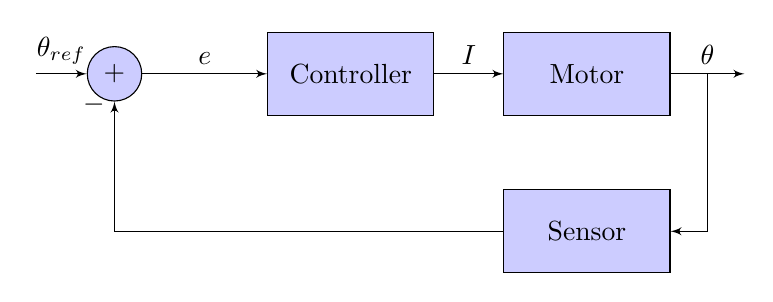
\begin{tikzpicture}[auto, node distance=2cm, >=latex']
    % Input
    \node [input, name=input] {};
    \node [sum, right of=input] (sum) {$+$};
    \node [block, right of=sum, node distance=3cm] (controller) {Controller};
    \node [block, right of=controller, node distance=3cm] (motor) {Motor};
    \node [output, right of=motor, node distance=2cm] (output) {};
    \node [block, below of=motor] (sensor) {Sensor};
    
    % Connections
    \draw [->] (input) -- node {$\theta_{ref}$} (sum);
    \draw [->] (sum) -- node {$e$} (controller);
    \draw [->] (controller) -- node {$I$} (motor);
    \draw [->] (motor) -- node [name=y] {$\theta$} (output);
    \draw [->] (y) |- (sensor);
    \draw [->] (sensor) -| node[pos=0.99] {$-$} (sum);
\end{tikzpicture}
\caption{Servo Motor Control System Block Diagram}
\end{figure}

\newpage

\section{Robotic Arm Joint System}

\subsection{System Description}

A robotic arm joint with moment of inertia $M$, friction coefficient $B$, and spring stiffness $k$ representing joint elasticity.

\subsection{Governing Equation}

\begin{equation}
M\ddot{\theta} + B\dot{\theta} + k\theta = \tau
\end{equation}

where:
\begin{itemize}
    \item $M$ = moment of inertia (kg·m²)
    \item $B$ = friction coefficient (N·m·s/rad)
    \item $k$ = spring stiffness (N·m/rad)
    \item $\tau$ = applied torque (N·m)
\end{itemize}

\subsection{Free Body Diagram}

\begin{figure}[H]
\centering
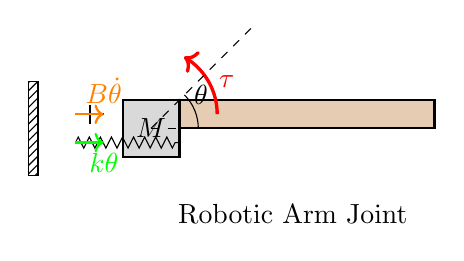
\begin{tikzpicture}[scale=1.2]
    % Joint representation
    \draw[thick, fill=gray!30] (-0.3,-0.3) rectangle (0.3,0.3);
    \node at (0,0) {$M$};
    
    % Arm segment
    \draw[thick, fill=brown!40] (0.3,0) -- (3,0) -- (3,0.3) -- (0.3,0.3) -- cycle;
    
    % Applied torque
    \draw[->, very thick, red] (0.7,0.15) arc (0:60:0.7) node[midway, right] {$\tau$};
    
    % Spring force
    \draw[decoration={zigzag,segment length=4pt,amplitude=2pt},decorate] (-0.8,-0.15) -- (0.3,-0.15);
    \draw[->, thick, green] (-0.8,-0.15) -- (-0.5,-0.15) node[below] {$k\theta$};
    
    % Damping force
    \draw[thick] (-0.8,0.15) -- (-0.5,0.15);
    \draw[thick] (-0.65,0.05) -- (-0.65,0.25);
    \draw[->, thick, orange] (-0.8,0.15) -- (-0.5,0.15) node[above] {$B\dot{\theta}$};
    
    % Angular position
    \draw[dashed] (0,0) -- (1.5,0);
    \draw[dashed] (0,0) -- (1.06,1.06);
    \draw (0.5,0) arc (0:45:0.5) node[right] {$\theta$};
    
    % Fixed support
    \draw[thick] (-1.2,-0.5) -- (-1.2,0.5);
    \draw[pattern=north east lines] (-1.3,-0.5) rectangle (-1.2,0.5);
    
    \node[below] at (1.5,-0.7) {Robotic Arm Joint};
\end{tikzpicture}
\caption{Free Body Diagram of Robotic Arm Joint}
\end{figure}

\subsection{Transfer Function}

\begin{equation}
G(s) = \frac{\Theta(s)}{\tau(s)} = \frac{1}{Ms^2 + Bs + k} = \frac{\omega_n^2}{s^2 + 2\zeta\omega_n s + \omega_n^2}
\end{equation}

where $\omega_n = \sqrt{k/M}$ and $\zeta = \frac{B}{2\sqrt{kM}}$

\subsection{Control System Block Diagram}

\begin{figure}[H]
\centering
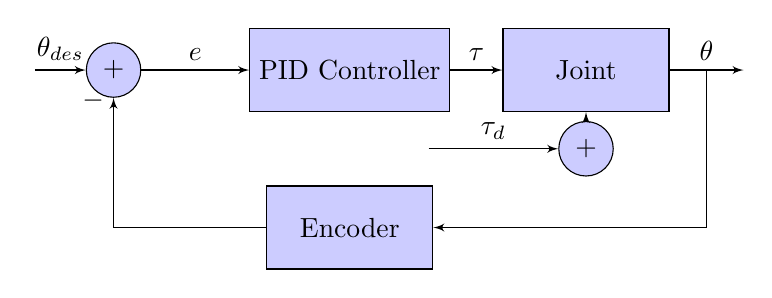
\begin{tikzpicture}[auto, node distance=2cm, >=latex']
    % Input
    \node [input, name=input] {};
    \node [sum, right of=input] (sum) {$+$};
    \node [block, right of=sum, node distance=3cm] (controller) {PID Controller};
    \node [block, right of=controller, node distance=3cm] (joint) {Joint};
    \node [output, right of=joint, node distance=2cm] (output) {};
    \node [sum, below of=joint] (disturbance) {$+$};
    \node [input, left of=disturbance] (dist_input) {};
    \node [block, below of=controller] (sensor) {Encoder};
    
    % Connections
    \draw [->] (input) -- node {$\theta_{des}$} (sum);
    \draw [->] (sum) -- node {$e$} (controller);
    \draw [->] (controller) -- node {$\tau$} (joint);
    \draw [->] (joint) -- node [name=y] {$\theta$} (output);
    \draw [->] (dist_input) -- node {$\tau_d$} (disturbance);
    \draw [->] (disturbance) -- (joint);
    \draw [->] (y) |- (sensor);
    \draw [->] (sensor) -| node[pos=0.99] {$-$} (sum);
\end{tikzpicture}
\caption{Robotic Arm Joint Control System Block Diagram}
\end{figure}

\newpage

\section{Ball Screw System}

\subsection{System Description}

A ball screw converts rotary motion to linear motion. The system has mass $M$, damping $B$, and experiences axial force $F$.

\subsection{Governing Equation}

\begin{equation}
M\ddot{x} + B\dot{x} = F
\end{equation}

where:
\begin{itemize}
    \item $M$ = mass (kg)
    \item $B$ = damping coefficient (N·s/m)
    \item $F$ = axial force (N)
    \item $x$ = position (m)
\end{itemize}

\subsection{Free Body Diagram}

\begin{figure}[H]
\centering
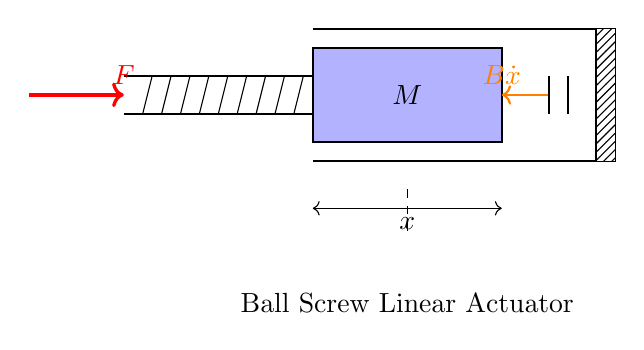
\begin{tikzpicture}[scale=1.2]
    % Mass block
    \draw[thick, fill=blue!30] (0,0) rectangle (2,1);
    \node at (1,0.5) {$M$};
    
    % Ball screw shaft
    \draw[thick] (-2,0.3) -- (0,0.3);
    \draw[thick] (-2,0.7) -- (0,0.7);
    
    % Ball screw thread representation
    \foreach \x in {-1.8,-1.6,...,-0.2} {
        \draw (\x,0.3) -- (\x+0.1,0.7);
    }
    
    % Applied force
    \draw[->, very thick, red] (-3,0.5) -- (-2,0.5) node[above] {$F$};
    
    % Damping force
    \draw[->, thick, orange] (2.5,0.5) -- (2,0.5) node[above] {$B\dot{x}$};
    \draw[thick] (2.7,0.3) -- (2.7,0.7);
    \draw[thick] (2.5,0.3) -- (2.5,0.7);
    
    % Position coordinate
    \draw[dashed] (1,-0.5) -- (1,-1);
    \draw[<->] (0,-0.7) -- (2,-0.7) node[midway, below] {$x$};
    
    % Fixed support
    \draw[thick] (3,-0.2) -- (3,1.2);
    \draw[pattern=north east lines] (3,-0.2) rectangle (3.2,1.2);
    
    % Rail guides
    \draw[thick] (0,-0.2) -- (3,-0.2);
    \draw[thick] (0,1.2) -- (3,1.2);
    
    \node[below] at (1,-1.5) {Ball Screw Linear Actuator};
\end{tikzpicture}
\caption{Free Body Diagram of Ball Screw System}
\end{figure}

\subsection{Transfer Functions}

Position output:
\begin{equation}
G_x(s) = \frac{X(s)}{F(s)} = \frac{1}{s(Ms + B)}
\end{equation}

Velocity output:
\begin{equation}
G_v(s) = \frac{sX(s)}{F(s)} = \frac{1}{Ms + B}
\end{equation}

\subsection{Control System Block Diagram}

\begin{figure}[H]
\centering
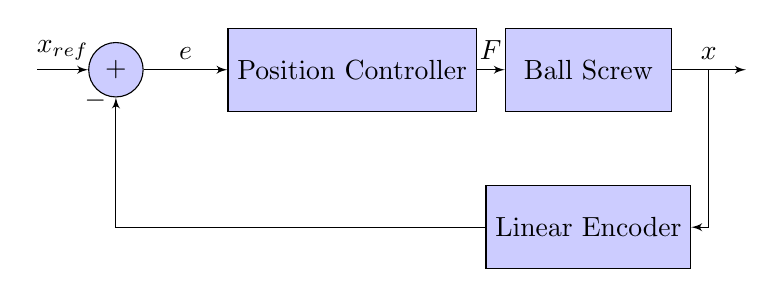
\begin{tikzpicture}[auto, node distance=2cm, >=latex']
    % Input
    \node [input, name=input] {};
    \node [sum, right of=input] (sum) {$+$};
    \node [block, right of=sum, node distance=3cm] (controller) {Position Controller};
    \node [block, right of=controller, node distance=3cm] (ballscrew) {Ball Screw};
    \node [output, right of=ballscrew, node distance=2cm] (output) {};
    \node [block, below of=ballscrew] (encoder) {Linear Encoder};
    
    % Connections
    \draw [->] (input) -- node {$x_{ref}$} (sum);
    \draw [->] (sum) -- node {$e$} (controller);
    \draw [->] (controller) -- node {$F$} (ballscrew);
    \draw [->] (ballscrew) -- node [name=y] {$x$} (output);
    \draw [->] (y) |- (encoder);
    \draw [->] (encoder) -| node[pos=0.99] {$-$} (sum);
\end{tikzpicture}
\caption{Ball Screw Control System Block Diagram}
\end{figure}

\newpage

\section{Conveyor Belt System}

\subsection{System Description}

A conveyor belt system with effective mass $M$, friction $B$, and drive force $F$ moving materials at velocity $v$.

\subsection{Governing Equation}

\begin{equation}
M\dot{v} + Bv = F
\end{equation}

where:
\begin{itemize}
    \item $M$ = effective mass of belt and load (kg)
    \item $B$ = friction coefficient (N·s/m)
    \item $F$ = drive force (N)
    \item $v$ = belt velocity (m/s)
\end{itemize}

\subsection{Free Body Diagram}

\begin{figure}[H]
\centering
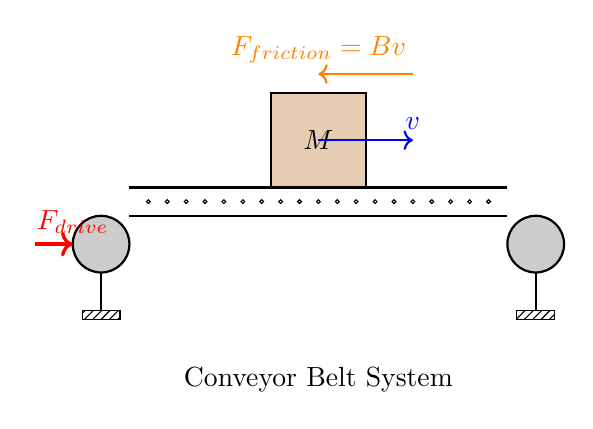
\begin{tikzpicture}[scale=1.2]
    % Belt representation
    \draw[thick] (0,0) -- (4,0);
    \draw[thick] (0,0.3) -- (4,0.3);
    
    % Pulleys
    \draw[thick, fill=gray!40] (-0.3,-0.3) circle (0.3);
    \draw[thick, fill=gray!40] (4.3,-0.3) circle (0.3);
    
    % Load on belt
    \draw[thick, fill=brown!40] (1.5,0.3) rectangle (2.5,1.3);
    \node at (2,0.8) {$M$};
    
    % Drive force
    \draw[->, very thick, red] (-1,-0.3) -- (-0.6,-0.3) node[above] {$F_{drive}$};
    
    % Friction force
    \draw[->, thick, orange] (3,1.5) -- (2,1.5) node[above] {$F_{friction} = Bv$};
    
    % Velocity vector
    \draw[->, thick, blue] (2,0.8) -- (3,0.8) node[above] {$v$};
    
    % Belt pattern
    \foreach \x in {0.2,0.4,...,3.8} {
        \draw (\x,0.15) circle (0.02);
    }
    
    % Support structure
    \draw[thick] (-0.3,-1) -- (-0.3,-0.6);
    \draw[thick] (4.3,-1) -- (4.3,-0.6);
    \draw[pattern=north east lines] (-0.5,-1) rectangle (-0.1,-1.1);
    \draw[pattern=north east lines] (4.1,-1) rectangle (4.5,-1.1);
    
    \node[below] at (2,-1.5) {Conveyor Belt System};
\end{tikzpicture}
\caption{Free Body Diagram of Conveyor Belt System}
\end{figure}

\subsection{Transfer Functions}

Velocity output:
\begin{equation}
G_v(s) = \frac{V(s)}{F(s)} = \frac{1}{Ms + B}
\end{equation}

Position output:
\begin{equation}
G_x(s) = \frac{X(s)}{F(s)} = \frac{1}{s(Ms + B)}
\end{equation}

\subsection{Control System Block Diagram}

\begin{figure}[H]
\centering
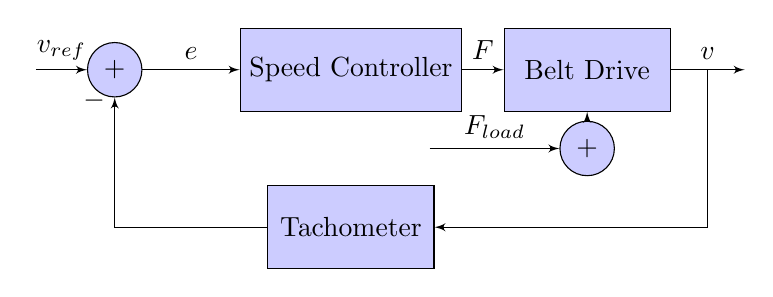
\begin{tikzpicture}[auto, node distance=2cm, >=latex']
    % Input
    \node [input, name=input] {};
    \node [sum, right of=input] (sum) {$+$};
    \node [block, right of=sum, node distance=3cm] (controller) {Speed Controller};
    \node [block, right of=controller, node distance=3cm] (belt) {Belt Drive};
    \node [output, right of=belt, node distance=2cm] (output) {};
    \node [sum, below of=belt] (load_sum) {$+$};
    \node [input, left of=load_sum] (load_input) {};
    \node [block, below of=controller] (tachometer) {Tachometer};
    
    % Connections
    \draw [->] (input) -- node {$v_{ref}$} (sum);
    \draw [->] (sum) -- node {$e$} (controller);
    \draw [->] (controller) -- node {$F$} (belt);
    \draw [->] (belt) -- node [name=y] {$v$} (output);
    \draw [->] (load_input) -- node {$F_{load}$} (load_sum);
    \draw [->] (load_sum) -- (belt);
    \draw [->] (y) |- (tachometer);
    \draw [->] (tachometer) -| node[pos=0.99] {$-$} (sum);
\end{tikzpicture}
\caption{Conveyor Belt Control System Block Diagram}
\end{figure}

\newpage

\section{Linear Actuator System}

\subsection{System Description}

A linear actuator with mass $M$, damping $B$, and spring constant $k$ representing mechanical compliance and stiffness.

\subsection{Governing Equation}

\begin{equation}
M\ddot{x} + B\dot{x} + kx = F
\end{equation}

where:
\begin{itemize}
    \item $M$ = mass (kg)
    \item $B$ = damping coefficient (N·s/m)
    \item $k$ = spring constant (N/m)
    \item $F$ = applied force (N)
    \item $x$ = position (m)
\end{itemize}

\subsection{Free Body Diagram}

\begin{figure}[H]
\centering
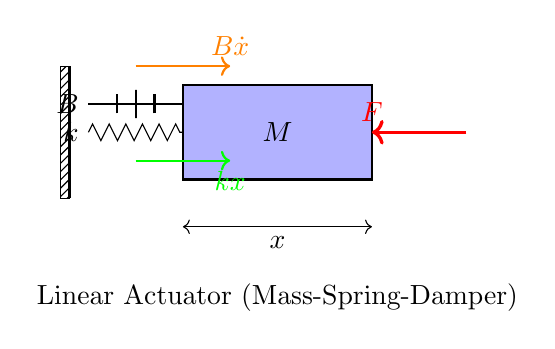
\begin{tikzpicture}[scale=1.2]
    % Mass
    \draw[thick, fill=blue!30] (1,0) rectangle (3,1);
    \node at (2,0.5) {$M$};
    
    % Spring
    \draw[decoration={zigzag,segment length=6pt,amplitude=3pt},decorate] (0,0.5) -- (1,0.5);
    \node[left] at (0,0.5) {$k$};
    
    % Damper
    \draw[thick] (0,0.8) -- (1,0.8);
    \draw[thick] (0.3,0.7) -- (0.3,0.9);
    \draw[thick] (0.7,0.7) -- (0.7,0.9);
    \draw[thick] (0.5,0.65) rectangle (0.5,0.95);
    \node[left] at (0,0.8) {$B$};
    
    % Applied force
    \draw[->, very thick, red] (4,0.5) -- (3,0.5) node[above] {$F$};
    
    % Spring force
    \draw[->, thick, green] (0.5,0.2) -- (1.5,0.2) node[below] {$kx$};
    
    % Damping force
    \draw[->, thick, orange] (0.5,1.2) -- (1.5,1.2) node[above] {$B\dot{x}$};
    
    % Position coordinate
    \draw[<->] (1,-0.5) -- (3,-0.5) node[midway, below] {$x$};
    
    % Fixed wall
    \draw[thick] (-0.2,-0.2) -- (-0.2,1.2);
    \draw[pattern=north east lines] (-0.3,-0.2) rectangle (-0.2,1.2);
    
    \node[below] at (2,-1) {Linear Actuator (Mass-Spring-Damper)};
\end{tikzpicture}
\caption{Free Body Diagram of Linear Actuator System}
\end{figure}

\subsection{Transfer Function}

\begin{equation}
G(s) = \frac{X(s)}{F(s)} = \frac{1}{Ms^2 + Bs + k} = \frac{\omega_n^2}{s^2 + 2\zeta\omega_n s + \omega_n^2}
\end{equation}

where $\omega_n = \sqrt{k/M}$ and $\zeta = \frac{B}{2\sqrt{kM}}$

\subsection{Control System Block Diagram}

\begin{figure}[H]
\centering
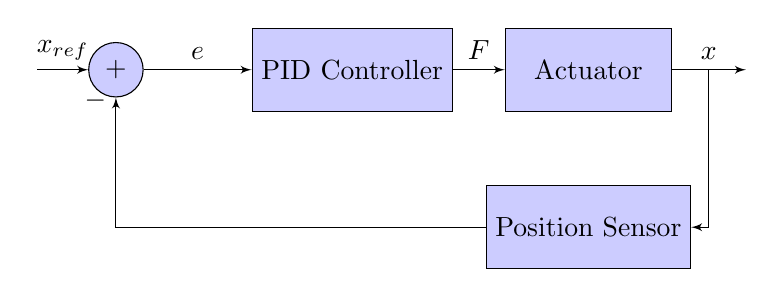
\begin{tikzpicture}[auto, node distance=2cm, >=latex']
    % Input
    \node [input, name=input] {};
    \node [sum, right of=input] (sum) {$+$};
    \node [block, right of=sum, node distance=3cm] (controller) {PID Controller};
    \node [block, right of=controller, node distance=3cm] (actuator) {Actuator};
    \node [output, right of=actuator, node distance=2cm] (output) {};
    \node [block, below of=actuator] (sensor) {Position Sensor};
    
    % Connections
    \draw [->] (input) -- node {$x_{ref}$} (sum);
    \draw [->] (sum) -- node {$e$} (controller);
    \draw [->] (controller) -- node {$F$} (actuator);
    \draw [->] (actuator) -- node [name=y] {$x$} (output);
    \draw [->] (y) |- (sensor);
    \draw [->] (sensor) -| node[pos=0.99] {$-$} (sum);
\end{tikzpicture}
\caption{Linear Actuator Control System Block Diagram}
\end{figure}

\newpage

\section{Wheel Drive System}

\subsection{System Description}

A wheel drive system with mass $M$, rolling resistance $B$, and traction force $F$ for vehicle motion.

\subsection{Governing Equation}

\begin{equation}
M\dot{v} + Bv = F
\end{equation}

where:
\begin{itemize}
    \item $M$ = vehicle mass (kg)
    \item $B$ = rolling resistance coefficient (N·s/m)
    \item $F$ = traction force (N)
    \item $v$ = velocity (m/s)
\end{itemize}

\subsection{Free Body Diagram}

\begin{figure}[H]
\centering
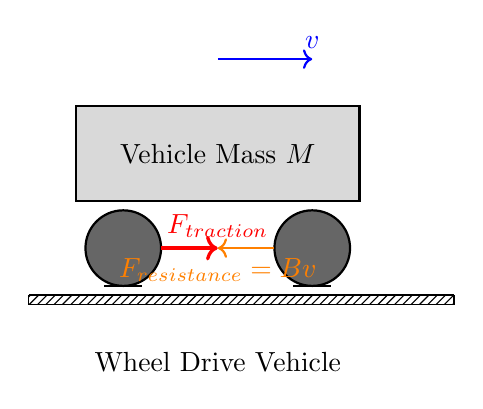
\begin{tikzpicture}[scale=1.2]
    % Vehicle body
    \draw[thick, fill=gray!30] (0,1) rectangle (3,2);
    \node at (1.5,1.5) {Vehicle Mass $M$};
    
    % Wheels
    \draw[thick, fill=black!60] (0.5,0.5) circle (0.4);
    \draw[thick, fill=black!60] (2.5,0.5) circle (0.4);
    
    % Traction force
    \draw[->, very thick, red] (0.9,0.5) -- (1.5,0.5) node[above] {$F_{traction}$};
    
    % Rolling resistance
    \draw[->, thick, orange] (2.1,0.5) -- (1.5,0.5) node[below] {$F_{resistance} = Bv$};
    
    % Velocity vector
    \draw[->, thick, blue] (1.5,2.5) -- (2.5,2.5) node[above] {$v$};
    
    % Ground contact
    \draw[thick] (-0.5,0) -- (4,0);
    \draw[pattern=north east lines] (-0.5,-0.1) rectangle (4,0);
    
    % Tire contact patches
    \draw[thick] (0.3,0.1) -- (0.7,0.1);
    \draw[thick] (2.3,0.1) -- (2.7,0.1);
    
    \node[below] at (1.5,-0.5) {Wheel Drive Vehicle};
\end{tikzpicture}
\caption{Free Body Diagram of Wheel Drive System}
\end{figure}

\subsection{Transfer Function}

\begin{equation}
G(s) = \frac{V(s)}{F(s)} = \frac{1}{Ms + B} = \frac{K}{\tau s + 1}
\end{equation}

where $K = 1/B$ and $\tau = M/B$

\subsection{Control System Block Diagram}

\begin{figure}[H]
\centering
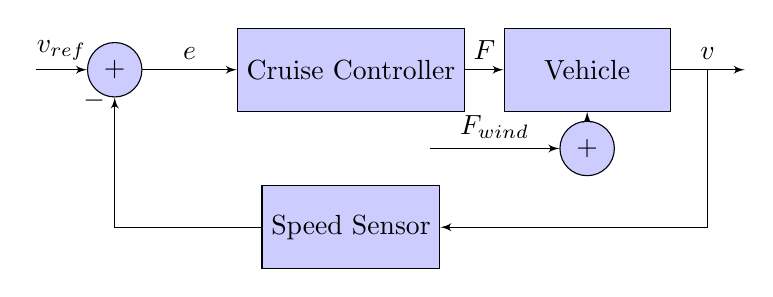
\begin{tikzpicture}[auto, node distance=2cm, >=latex']
    % Input
    \node [input, name=input] {};
    \node [sum, right of=input] (sum) {$+$};
    \node [block, right of=sum, node distance=3cm] (controller) {Cruise Controller};
    \node [block, right of=controller, node distance=3cm] (vehicle) {Vehicle};
    \node [output, right of=vehicle, node distance=2cm] (output) {};
    \node [sum, below of=vehicle] (dist_sum) {$+$};
    \node [input, left of=dist_sum] (dist_input) {};
    \node [block, below of=controller] (speedometer) {Speed Sensor};
    
    % Connections
    \draw [->] (input) -- node {$v_{ref}$} (sum);
    \draw [->] (sum) -- node {$e$} (controller);
    \draw [->] (controller) -- node {$F$} (vehicle);
    \draw [->] (vehicle) -- node [name=y] {$v$} (output);
    \draw [->] (dist_input) -- node {$F_{wind}$} (dist_sum);
    \draw [->] (dist_sum) -- (vehicle);
    \draw [->] (y) |- (speedometer);
    \draw [->] (speedometer) -| node[pos=0.99] {$-$} (sum);
\end{tikzpicture}
\caption{Wheel Drive Control System Block Diagram}
\end{figure}

\newpage

\section{Gearbox System}

\subsection{System Description}

A gearbox with input and output inertias, gear ratio $N$, and various compliance and damping effects.

\subsection{Governing Equations}

Input side:
\begin{equation}
J_1\ddot{\theta_1} + B_1\dot{\theta_1} + K(\theta_1 - N\theta_2) = \tau_1
\end{equation}

Output side:
\begin{equation}
J_2\ddot{\theta_2} + B_2\dot{\theta_2} + K(\theta_2 - \frac{\theta_1}{N}) = \frac{\tau_L}{N}
\end{equation}

where:
\begin{itemize}
    \item $J_1, J_2$ = input and output inertias (kg·m²)
    \item $B_1, B_2$ = input and output damping (N·m·s/rad)
    \item $K$ = shaft stiffness (N·m/rad)
    \item $N$ = gear ratio
    \item $\tau_1$ = input torque, $\tau_L$ = load torque
\end{itemize}

\subsection{Free Body Diagram}

\begin{figure}[H]
\centering
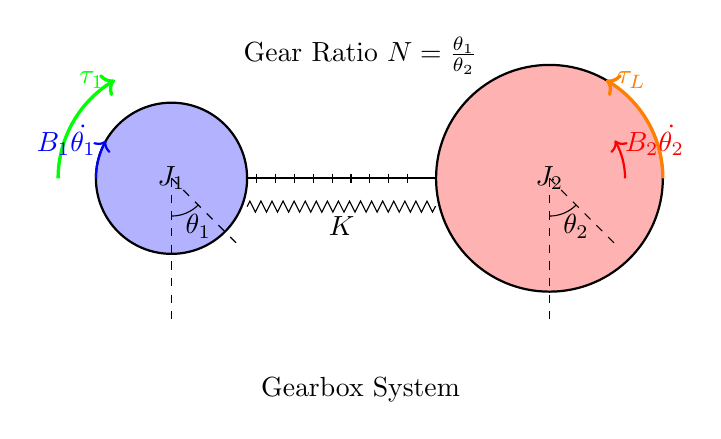
\begin{tikzpicture}[scale=1.2]
    % Input gear (small)
    \draw[thick, fill=blue!30] (-2,0) circle (0.8);
    \node at (-2,0) {$J_1$};
    
    % Output gear (large)
    \draw[thick, fill=red!30] (2,0) circle (1.2);
    \node at (2,0) {$J_2$};
    
    % Gear teeth engagement
    \draw[thick] (-1.2,0) -- (0.8,0);
    \foreach \x in {-1.1,-0.9,...,0.7} {
        \draw (\x,0.05) -- (\x,-0.05);
    }
    
    % Input torque
    \draw[->, very thick, green] (-3.2,0) arc (180:120:1.2) node[left] {$\tau_1$};
    
    % Output torque
    \draw[->, very thick, orange] (3.2,0) arc (0:60:1.2) node[right] {$\tau_L$};
    
    % Input damping
    \draw[->, thick, blue] (-2.8,0) arc (180:150:0.8) node[left] {$B_1\dot{\theta_1}$};
    
    % Output damping
    \draw[->, thick, red] (2.8,0) arc (0:30:0.8) node[right] {$B_2\dot{\theta_2}$};
    
    % Shaft compliance (spring)
    \draw[decoration={zigzag,segment length=4pt,amplitude=2pt},decorate] (-1.2,-0.3) -- (0.8,-0.3);
    \node[below] at (-0.2,-0.3) {$K$};
    
    % Angular positions
    \draw[dashed] (-2,0) -- (-2,-1.5);
    \draw[dashed] (-2,0) -- (-1.3,-0.7);
    \draw (-2,-0.4) arc (270:315:0.4) node[below] {$\theta_1$};
    
    \draw[dashed] (2,0) -- (2,-1.5);
    \draw[dashed] (2,0) -- (2.7,-0.7);
    \draw (2,-0.4) arc (270:315:0.4) node[below] {$\theta_2$};
    
    % Gear ratio indication
    \node[above] at (0,1) {Gear Ratio $N = \frac{\theta_1}{\theta_2}$};
    
    \node[below] at (0,-2) {Gearbox System};
\end{tikzpicture}
\caption{Free Body Diagram of Gearbox System}
\end{figure}

\subsection{Control System Block Diagram}

\begin{figure}[H]
\centering
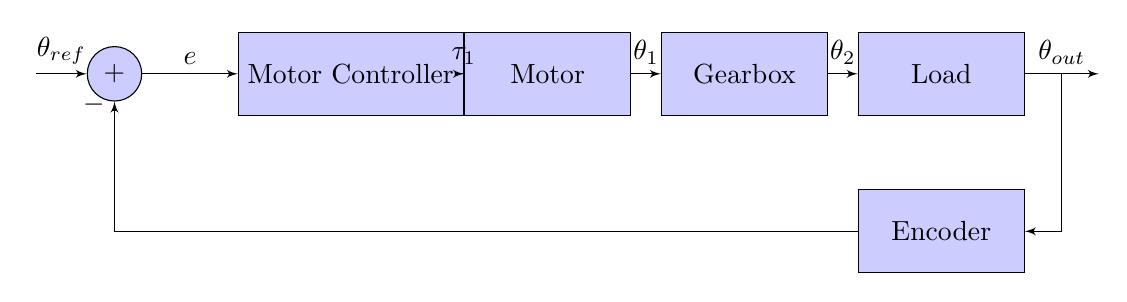
\begin{tikzpicture}[auto, node distance=2cm, >=latex']
    % Input
    \node [input, name=input] {};
    \node [sum, right of=input] (sum) {$+$};
    \node [block, right of=sum, node distance=3cm] (controller) {Motor Controller};
    \node [block, right of=controller, node distance=2.5cm] (motor) {Motor};
    \node [block, right of=motor, node distance=2.5cm] (gearbox) {Gearbox};
    \node [block, right of=gearbox, node distance=2.5cm] (load) {Load};
    \node [output, right of=load, node distance=2cm] (output) {};
    \node [block, below of=load] (encoder) {Encoder};
    
    % Connections
    \draw [->] (input) -- node {$\theta_{ref}$} (sum);
    \draw [->] (sum) -- node {$e$} (controller);
    \draw [->] (controller) -- node {$\tau_1$} (motor);
    \draw [->] (motor) -- node {$\theta_1$} (gearbox);
    \draw [->] (gearbox) -- node {$\theta_2$} (load);
    \draw [->] (load) -- node [name=y] {$\theta_{out}$} (output);
    \draw [->] (y) |- (encoder);
    \draw [->] (encoder) -| node[pos=0.99] {$-$} (sum);
\end{tikzpicture}
\caption{Gearbox Control System Block Diagram}
\end{figure}

\newpage

\section{Summary Table}

\begin{table}[H]
\centering
\caption{Summary of System Transfer Functions}
\begin{tabular}{|l|c|c|c|}
\hline
\textbf{System} & \textbf{Order} & \textbf{Transfer Function} & \textbf{Characteristics} \\
\hline
Servo Motor & 2nd & $\frac{K_t}{Js^2 + Ds}$ & Integrator + 1st order \\
\hline
Robot Joint & 2nd & $\frac{1}{Ms^2 + Bs + k}$ & Second order \\
\hline
Ball Screw & 2nd & $\frac{1}{s(Ms + B)}$ & Integrator + 1st order \\
\hline
Conveyor Belt & 1st & $\frac{1}{Ms + B}$ & First order \\
\hline
Linear Actuator & 2nd & $\frac{1}{Ms^2 + Bs + k}$ & Second order \\
\hline
Wheel Drive & 1st & $\frac{1}{Ms + B}$ & First order \\
\hline
Gearbox & 4th & Complex multi-body & Flexible coupling \\
\hline
\end{tabular}
\end{table}

\section{Design Considerations}

\subsection{Stability Analysis}
Each system's stability depends on pole locations:
\begin{itemize}
    \item \textbf{First-order systems}: Always stable if $B > 0$
    \item \textbf{Second-order systems}: Stable if $B > 0$ and $k > 0$
    \item \textbf{Integrator systems}: Marginally stable, require feedback for stability
\end{itemize}

\subsection{Performance Metrics}
Key performance metrics for each system type:
\begin{itemize}
    \item \textbf{Rise time}: $t_r \approx \frac{1.8}{\omega_n}$ for second-order systems
    \item \textbf{Settling time}: $t_s \approx \frac{4}{\zeta\omega_n}$ for second-order systems
    \item \textbf{Overshoot}: $MP = 100e^{-\frac{\pi\zeta}{\sqrt{1-\zeta^2}}}$ \% for $\zeta < 1$
    \item \textbf{Steady-state error}: Depends on system type and input
\end{itemize}

\subsection{Control Strategy Selection}
\begin{itemize}
    \item \textbf{PID Control}: Suitable for most systems with proper tuning
    \item \textbf{Lead/Lag Compensation}: For specific frequency domain requirements
    \item \textbf{State Feedback}: For multi-input multi-output systems
    \item \textbf{Adaptive Control}: For systems with parameter variations
\end{itemize}

\section{Conclusion}

This document provides comprehensive free body diagrams and control system representations for common mechanical systems. The mathematical models serve as the foundation for control system design, analysis, and implementation. Understanding these fundamental systems enables engineers to design effective control strategies for complex multi-body systems.

\end{document}